\documentclass[
11pt, % The default document font size, options: 10pt, 11pt, 12pt
codirector, % Uncomment to add a codirector to the title page
]{charter} 


% El títulos de la memoria, se usa en la carátula y se puede usar el cualquier lugar del documento con el comando \ttitle
\titulo{Aplicación web para el control de acceso en alquileres temporales mediante la gestión de periféricos} 
% Nombre del posgrado, se usa en la carátula y se puede usar el cualquier lugar del documento con el comando \degreename
\posgrado{Carrera de Especialización en Sistemas Embebidos} 
%\posgrado{Carrera de Especialización en Internet de las Cosas} 
%\posgrado{Carrera de Especialización en Inteligencia Artificial}
%\posgrado{Maestría en Sistemas Embebidos} 
%\posgrado{Maestría en Internet de las cosas}
% IMPORTANTE: no omitir titulaciones ni tildación en los nombres, también se recomienda escribir los nombres completos (tal cual los tienen en su documento)
% Tu nombre, se puede usar el cualquier lugar del documento con el comando \authorname
\autor{Ing. Andrea García}

% El nombre del director y co-director, se puede usar el cualquier lugar del documento con el comando \supname y \cosupname y \pertesupname y \pertecosupname
\director{Ing. Sergio Starkloff, CTO}
\pertenenciaDirector{SURiX} 
\codirector{} % para que aparezca en la portada se debe descomentar la opción codirector en los parámetros de documentclass
\pertenenciaCoDirector{FIUBA}

% Nombre del cliente, quien va a aprobar los resultados del proyecto, se puede usar con el comando \clientename y \empclientename
\cliente{Ing. Sergio Starkloff, CTO}
\empresaCliente{SURiX}
 
\fechaINICIO{27 de febrero de 2024}		%Fecha de inicio de la cursada de GdP \fechaInicioName
\fechaFINALPlan{16 de abril de 2024} 	%Fecha de final de cursada de GdP
\fechaFINALTrabajo{xx de mayo de 2024}	%Fecha de defensa pública del trabajo final

\usepackage{rotating}

\begin{document}

\maketitle
\thispagestyle{empty}
\pagebreak


\thispagestyle{empty}
{\setlength{\parskip}{0pt}
\tableofcontents{}
}
\pagebreak


\section*{Registros de cambios}
\label{sec:registro}


\begin{table}[ht]
\label{tab:registro}
\centering
\begin{tabularx}{\linewidth}{@{}|c|X|c|@{}}
\hline
\rowcolor[HTML]{C0C0C0} 
Revisión & \multicolumn{1}{c|}{\cellcolor[HTML]{C0C0C0}Detalles de los cambios realizados} & Fecha      \\ \hline
0      & Creación del documento                                 &\fechaInicioName \\ \hline
1      & Se completa hasta el punto 5 inclusive                & 12 de marzo de 2024 \\ \hline
2      & Se completa hasta el punto 9 inclusive                & 19 de marzo de 2024 \\ \hline
3      & Se completa hasta el punto 12 inclusive                & 26 de marzo de 2024 \\ \hline
%4      & Se completa el plan	                                 & {día} de {mes} de 202X \\ \hline

% Si hay más correcciones pasada la versión 4 también se deben especificar acá

\end{tabularx}
\end{table}

\pagebreak



\section*{Acta de constitución del proyecto}
\label{sec:acta}

\begin{flushright}
Buenos Aires, \fechaInicioName
\end{flushright}

\vspace{2cm}

Por medio de la presente se acuerda con la \authorname\hspace{1px} que su Trabajo Final de la \degreename\hspace{1px} se titulará ``\ttitle'' y consistirá en desarrollar una aplicación web en colaboración con SURiX para facilitar el ingreso a propiedades rentadas por periodos cortos mediante la interacción con dispositivos móviles de los inquilinos. El trabajo tendrá un presupuesto preliminar estimado de \textcolor{red}{600} horas y un costo estimado de \textcolor{red}{\$ XXX}, con fecha de inicio el \fechaInicioName\hspace{1px} y fecha de presentación pública el \fechaFinalName.

Se adjunta a esta acta la planificación inicial.

\vfill

% Esta parte se construye sola con la información que hayan cargado en el preámbulo del documento y no debe modificarla
\begin{table}[ht]
\centering
\begin{tabular}{ccc}
\begin{tabular}[c]{@{}c@{}}Dr. Ing. Ariel Lutenberg \\ Director posgrado FIUBA\end{tabular} & \hspace{2cm} & \begin{tabular}[c]{@{}c@{}}\clientename \\ \empclientename \end{tabular} \vspace{2.5cm} \\ 
\multicolumn{3}{c}{\begin{tabular}[c]{@{}c@{}} \supname \\ Director del Trabajo Final\end{tabular}} \vspace{2.5cm} \\
\end{tabular}
\end{table}




\section{1. Descripción técnica-conceptual del proyecto a realizar}
\label{sec:descripcion}

El proyecto actual forma parte del programa de vinculación de la Universidad de Buenos Aires en colaboración con SURiX, una empresa líder con más de dos décadas de experiencia en soluciones IP para seguridad y control de acceso. La motivación para abordar la interacción de periféricos desde la web surge como respuesta a la ineficiencia detectada en la coordinación de la entrega de llaves, una problemática evidente en el ámbito de la renta de alojamientos colaborativos como Airbnb.

La solución propuesta se basa en una aplicación que utiliza tecnología web para ofrecer una experiencia eficiente, segura y cómoda, permitiendo el acceso a través de los periféricos de los dispositivos móviles de los usuarios. El proceso se divide en cuatro fases: integración con las APIs de Bluetooth y grabación de audio, diseño y desarrollo de la página web, pruebas y ajustes, y finalmente, la implementación y lanzamiento del sistema.

En el ámbito comercial, las cerraduras digitales son comúnmente utilizadas para transformar la seguridad residencial en este ámbito. Sin embargo, la presente iniciativa está basada en la web y se destaca por su enfoque en la accesibilidad e interoperabilidad, a diferencia de los dispositivos que a menudo requieren aplicaciones propias. El contar con un aplicativo privado constituye una restricción, ya que suele depender de las actualizaciones del sistema operativo, además la creciente variedad de dispositivos puede generar desafíos en términos de compatibilidad y desarrollo.

La lógica de funcionamiento del proyecto en mención utiliza recursos web para interactuar con la cámara, Bluetooth y audio del teléfono móvil del inquilino. Esto permite acciones como el escaneo de códigos QR, validación de información, apertura de puertas, comunicación a través de bluetooth y un buzón de voz para mensajes entre inquilino y propietario tal como se muestra en la figura \ref{fig:diagBloques}. La facilidad de uso, interfaz intuitiva y accesibilidad universal resaltan la singularidad del proyecto, respaldado por la experiencia de SURiX en soluciones tecnológicas innovadoras.

\begin{figure}[htpb]
\centering 
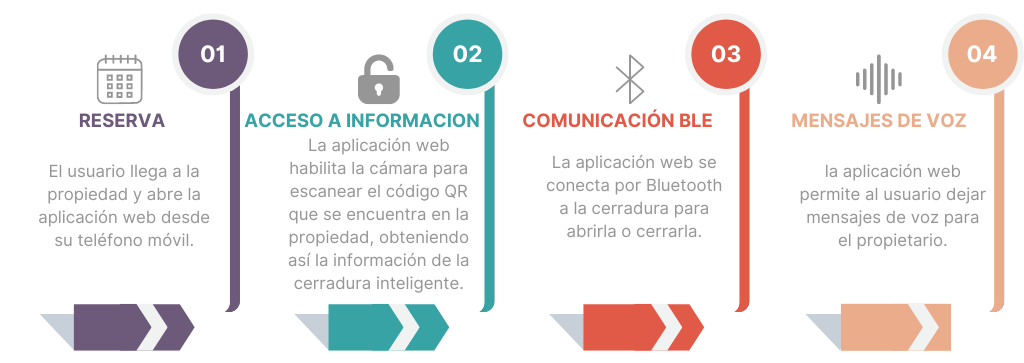
\includegraphics[width=1\textwidth]{./Figuras/flowchart.png}
\caption{Diagrama en bloques del sistema.}
\label{fig:diagBloques}
\end{figure}

Este prototipo, si bien integra la aplicación web con periféricos del teléfono, no involucra bases de datos para inquilinos o propietarios y carece de controles temporales para el acceso. Asimismo, prescinde de un sistema de inicio de sesión y, en relación al buzón de voz, propone un modelo donde los mensajes del usuario se convierten en mensajes recibidos lo que establece un ciclo continuo. Este diseño simplificado concuerda con el propósito demostrativo del proyecto, enfocándose en la esencial interacción web-periférico.  

\section{2. Identificación y análisis de los interesados}
\label{sec:interesados}

Para llevar a cabo este proyecto de colaboración entre la empresa asociada y la UBA, se requiere la participación de varios individuos. A continuación en el cuadro \ref{tab:interesados}, se detalla a los involucrados:
\begin{table}[ht]
\caption{Identificación de los interesados}
\label{tab:interesados}
\begin{tabularx}{\linewidth}{@{}|l|X|X|l|@{}}
\hline
\rowcolor[HTML]{C0C0C0} 
Rol           & Nombre y Apellido & Organización 	& Puesto 	\\ \hline
%Auspiciante   &        -          &        -        &         -          \\ \hline
Cliente       & SURiX      &\empclientename	& Empresa de vinculación\\ \hline
%Impulsor      &        -          &        -        &        	\\ \hline
Responsable   & \authorname       & FIUBA        	& Alumno 	\\ \hline
%Colaboradores &        -          &        -        &        -          \\ \hline
Orientador    & \clientename      &\empclientename	& Director del Trabajo Final\\ \hline
Equipo        & Leslie Queglas \newline 
			Estefanía Del Valle Fiorabanti & SURiX &Full Stack Developers\\ \hline
%Opositores    &        -          &         -       &        -          \\ \hline
%Usuario final &        -          &         -       &        -          \\ \hline
\end{tabularx}
\end{table}

\begin{itemize}
        \item Cliente: SURIX, fundada en 1998, es una empresa que ofrece soluciones de comunicación y control de acceso IP y analógico.
        \item Responsable: Andrea García, es la persona encargada del desarrollo del aplicativo web y la realización de pruebas.
	\item Orientador: Sergio Starkloff, fundador de SURiX, lidera la propuesta en calidad de director del trabajo final. Define los requisitos tecnológicos clave para resolver la problemática central del proyecto.
	\item Equipo: los miembros del equipo, Leslie Quetglas y Estefanıa Del Valle Fiorabanti, forman parte de SURiX como desarrolladoras Full Stack y apoyan a la responsable en temas de Front End del presente proyecto.
	
\end{itemize}

\section{3. Propósito del proyecto}
\label{sec:proposito}

El propósito de este proyecto es abordar la ineficiencia en la coordinación de la entrega de llaves en el alquiler de alojamientos temporarios, mediante el desarrollo de una aplicación web innovadora que permita el acceso a través de los dispositivos móviles de los usuarios, interactuando con los periféricos correspondientes. Se busca mejorar la experiencia de los usuarios y optimizar la gestión de las propiedades, ofreciendo una solución integral basada en la accesibilidad, interoperabilidad y seguridad proporcionadas por la tecnología web.
\newpage
\section{4. Alcance del proyecto}
\label{sec:alcance}

El proyecto incluye:
\begin{itemize}
	\item Desarrollo de una aplicación web para la gestión de acceso a alojamientos temporarios.
        \begin{itemize}
    		\item Integración con APIs de Bluetooth y grabación de audio.
    		\item Diseño y desarrollo de la interfaz de usuario.
        \end{itemize}
	\item Pruebas y ajustes del sistema.
\end{itemize}

El proyecto no incluye:
\begin{itemize}
	\item Implementación de una base de datos para gestionar información de inquilinos o propietarios.
        \item Control de fechas y horarios para el acceso.
        \item Sistema de inicio de sesión.
	\item Desarrollo de hardware para dispositivos de acceso.
\end{itemize}

\section{5. Supuestos del proyecto}
\label{sec:supuestos}
Para el desarrollo del presente proyecto se supone que:

\begin{itemize}
	\item Se dispone del equipo necesario para llevar a cabo pruebas de comunicación entre periféricos y hardware, lo cual incluye dispositivos móviles compatibles con Bluetooth y acceso a servidores propios proporcionados por SURiX para alojar la aplicación web.
	\item Existe acceso a herramientas de desarrollo de software y entornos de prueba para garantizar la funcionalidad y compatibilidad del sistema en diferentes dispositivos móviles.
	\item Se cuenta con un ambiente de pruebas adecuado para simular escenarios de uso real y verificar la interoperabilidad de los periféricos con la aplicación web.
        \item El personal técnico tiene el conocimiento y la capacitación necesarios para llevar a cabo las pruebas de manera efectiva y resolver cualquier problema que pueda surgir durante el proceso de desarrollo.
\end{itemize}

\section{6. Requerimientos}

\subsection{Requerimientos funcionales}
\begin{enumerate}
\item Los usuarios deben poder visualizar la información de la propiedad correspondiente para alquiler temporal (prioridad menor).
\item Los usuarios deben poder utilizar los periféricos de su teléfono móvil para interactuar con la aplicación (prioridad mayor).
\item La aplicación web debe proporcionar una funcionalidad de escaneo de códigos QR para acceder a la información de la propiedad (prioridad mayor).
\item Una vez escaneado el código QR, la aplicación debe proporcionar al usuario la información necesaria para conectarse por Bluetooth con la cerradura electrónica de la propiedad (prioridad mayor).
\item La aplicación debe permitir al usuario abrir o cerrar la cerradura electrónica utilizando la funcionalidad de activación Bluetooth (prioridad mayor).
\item El sistema debe notificar al propietario cuando la cerradura electrónica se abre o se cierra (prioridad menor).
\item La aplicación web debe facilitar la comunicación entre el inquilino y el propietario mediante mensajes de voz (prioridad mayor).
\item La aplicación debe ser compatible con el navegador web Chrome con versión mínima 85 en sistema operativo Android (prioridad mayor).
\item Todos los mensajes de voz y la información relacionada deben estar alojados en los servidores de SURiX (prioridad menor).
\end{enumerate}

\subsection{Requerimientos de documentación}
\begin{enumerate}
\item Se debe incluir un manual de usuario que explique cómo utilizar todas las funciones de la aplicación (prioridad mayor).
\item La documentación técnica debe describir la arquitectura del sistema y los requisitos de hardware y software necesarios para su implementación (prioridad menor).
\end{enumerate}

\subsection{Requerimientos de testing}
\begin{enumerate}
\item Se deben realizar pruebas exhaustivas de funcionalidad para asegurar que todas las características de la aplicación funcionen correctamente (prioridad mayor).
\item Se deben llevar a cabo pruebas de compatibilidad para verificar que la aplicación sea compatible con determinados dispositivos móviles y navegadores web (prioridad mayor).
\item Se deben realizar pruebas de seguridad para identificar posibles vulnerabilidades y asegurar la protección de los datos de los usuarios (prioridad menor).
\end{enumerate}

\subsection{Requerimientos de interfaz}
\begin{enumerate}
\item La interfaz de usuario debe ser intuitiva y fácil de navegar (prioridad mayor).
\item Se debe proporcionar retroalimentación visual para confirmar las acciones realizadas por el usuario, como el acceso a la propiedad o el envío de un mensaje de voz (prioridad menor).
\item La aplicación debe contar con un diseño \textit{responsive} que se adapte automáticamente a diferentes tamaños de pantalla (prioridad menor).
\end{enumerate}

\section{7. Historias de usuarios (\textit{Product backlog})}
\label{sec:backlog}

\subsection{Roles}
\begin{itemize}
\item Inquilino: usuario que alquila una propiedad temporalmente y necesita acceder a través de la aplicación web.
\item Propietario: usuario que ofrece propiedades en alquiler temporal y necesita gestionar el acceso de los inquilinos.
\end{itemize}

\subsection{Puntos de historia}
Para la ponderación de cada historia de usuario, se hará uso de una escala que comprende valores entre 1, 2, 3 y 5. En el caso de que una de ellas llegara a ser calificada con 5, daría lugar a una nueva tarea en el plan de proyecto que puede ser ejecutada como un \textit{sprint} de no más de 40 horas.

La asignación de puntos es relativa a tres ejes: funcionamiento, complejidad y dificultad. La prioridad es valorada según el número de historias y los puntos de cada una.

\begin{itemize}
\item 1 punto: requiere modificaciones mínimas en el sistema y no demanda muchas horas de desarrollo.
\item 2 puntos: requiere cambios en el sistema y demanda varias horas de desarrollo.
\item 3 puntos: implica riesgo de modificar el sistema y puede demandar muchas horas de desarrollo.
\item 5 puntos: si la funcionalidad no se implementa, el sistema no funciona correctamente.
\end{itemize}
\subsection{Historias de usuarios}
\begin{table}[h]
\centering
\begin{tabular}{|c|c|c|} 
\hline
\textbf{Historia de usuario}                                                                                                                                                                                                                                      & \begin{tabular}[c]{@{}c@{}}\textbf{Puntos de}\\\textbf{historia}\end{tabular} & \multicolumn{1}{l|}{\textbf{Prioridad}}  \\ 
\hline
\begin{tabular}[c]{@{}c@{}}Como inquilino/a, quiero visualizar la información detallada\\ de la propiedad que he reservado para conocer los detalles\\relevantes antes de mi llegada.\end{tabular}                                                                              & 1                                                                             & 4                                        \\ 
\hline
\begin{tabular}[c]{@{}c@{}}Como inquilino/a, deseo utilizar la aplicación web para\\ acceder a la propiedad reservada mediante los\\periféricos de mi teléfono móvil.\end{tabular} & 5                                                                             & 1                                        \\ 
\hline
\begin{tabular}[c]{@{}c@{}}Como propietario/a, necesito recibir notificaciones\\cuando un inquilino acceda o salga de la propiedad para\\mantener un registro de los accesos.\end{tabular}                                   & 2                                                                             & 3                                        \\ 
\hline
\begin{tabular}[c]{@{}c@{}}Como inquilino/a, quiero poder comunicarme con el\\ propietario mediante mensajes de voz integrados en la aplicación\\web para resolver cualquier consulta o inconveniente durante mi estadía.\end{tabular}                                                                          & 3                                                                             & 2                                        \\
\hline
\end{tabular}
\end{table}

\section{8. Entregables principales del proyecto}
\label{sec:entregables}

Los entregables del proyecto son:

\begin{itemize}
    \item Manual de usuario detallado que explique cómo utilizar todas las funciones de la aplicación, incluyendo la interacción con los periféricos móviles y la gestión de accesos a propiedades temporales.
    \item Documentación técnica que describa la arquitectura del sistema, los requisitos de hardware y software, y los procedimientos de instalación y configuración.
    \item Código fuente de la aplicación web, que incluya todas las funcionalidades requeridas, como el escaneo de códigos QR, la activación Bluetooth de la cerradura electrónica y la comunicación por mensajes de voz.
    \item Informe de pruebas que detalle los resultados de las pruebas de funcionalidad, compatibilidad y seguridad realizadas para garantizar el correcto funcionamiento.
\end{itemize}

\section{9. Desglose del trabajo en tareas}
\label{sec:wbs}
\begin{enumerate}
\item Desarrollo de la aplicación web (250 h)
\begin{enumerate}
    \item Investigación y selección de tecnologías (40 h)
    \item Diseño de la arquitectura (40 h)
    \item Implementación de la funcionalidad de visualización de información de la propiedad (20 h)
    \item Desarrollo de la funcionalidad de escaneo de códigos QR (30 h)
    \item Desarrollo de la funcionalidad de activación Bluetooth (30 h)
    \item Desarrollo de la funcionalidad de grabar, guardar y enviar audio (90 h)
\end{enumerate}
\item Pruebas y ajustes (180 h)
\begin{enumerate}
    \item Realización de pruebas de funcionalidad (70 h)
    \item Ejecución de pruebas de compatibilidad (50 h)
    \item Realización de pruebas de seguridad (60 h)
\end{enumerate}

\item Documentación (90 h)
\begin{enumerate}
    \item Elaboración del manual de usuario (40 h)
    \item Redacción de la documentación técnica (50 h)
\end{enumerate}

\item Preparación de entregables finales (70 h)
\begin{enumerate}
    \item Elaboración del informe de pruebas (20 h)
    \item Redacción de la memoria del trabajo final (50 h)
\end{enumerate}
\end{enumerate}

Cantidad total de horas: 590 h.

\section{10. Diagrama de Activity On Node}
\label{sec:AoN}
Para poder identificar el flujo secuencial de las tareas del proyecto se ilustra un diagrama AON (\textit{Activity On Node}) (Véase Figura \ref{fig:AoN.drawio.png}). La ruta crítica es resaltada con bordes en negrita y posee una duración de 370 hs.

\begin{figure}[htpb]
\centering 
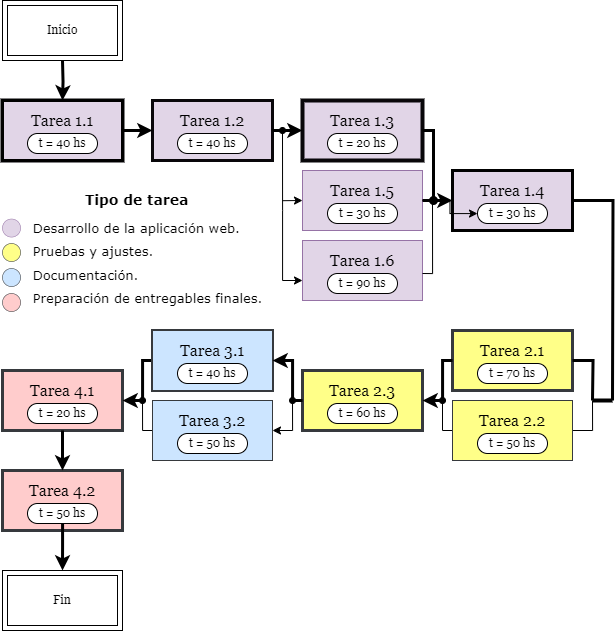
\includegraphics[width=.9\textwidth]{./Figuras/AON.drawio.png}
\caption{Diagrama en \textit{Activity on Node.}}
\label{fig:AoN}
\end{figure}

\section{11. Diagrama de Gantt}
\label{sec:gantt}
En la Figura \ref{fig:Tasks} se encuentran las tareas listadas con su fecha de inicio y fin según su organización a través de la apliación web Online Gantt. La representación gráfica en línea de tiempo puede ser observada en la Figura \ref{fig:Gantt}.
\begin{figure}[htpb]
\centering 
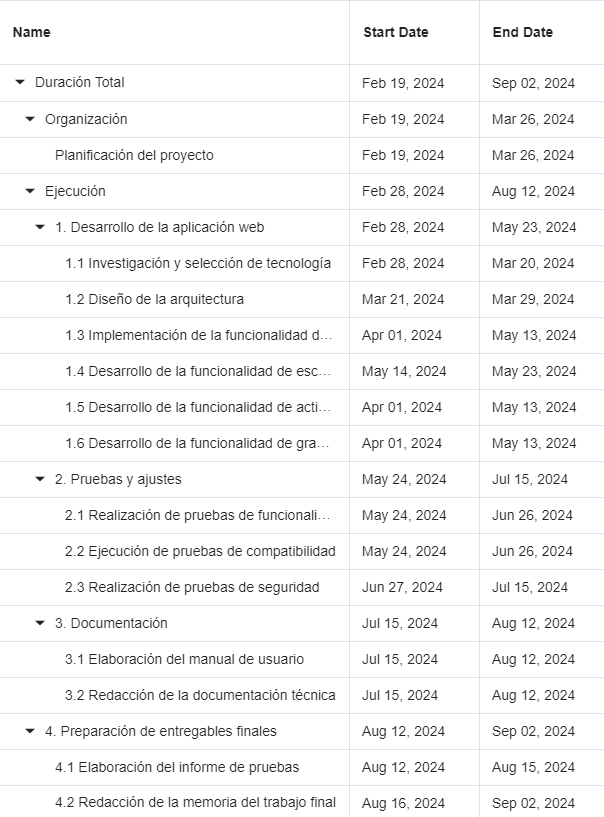
\includegraphics[width=.9\textwidth]{./Figuras/tareas.png}
\caption{Tareas del plan de proyecto.}
\label{fig:Tasks}
\end{figure}

\begin{sidewaysfigure}[htpb]
    \centering 
    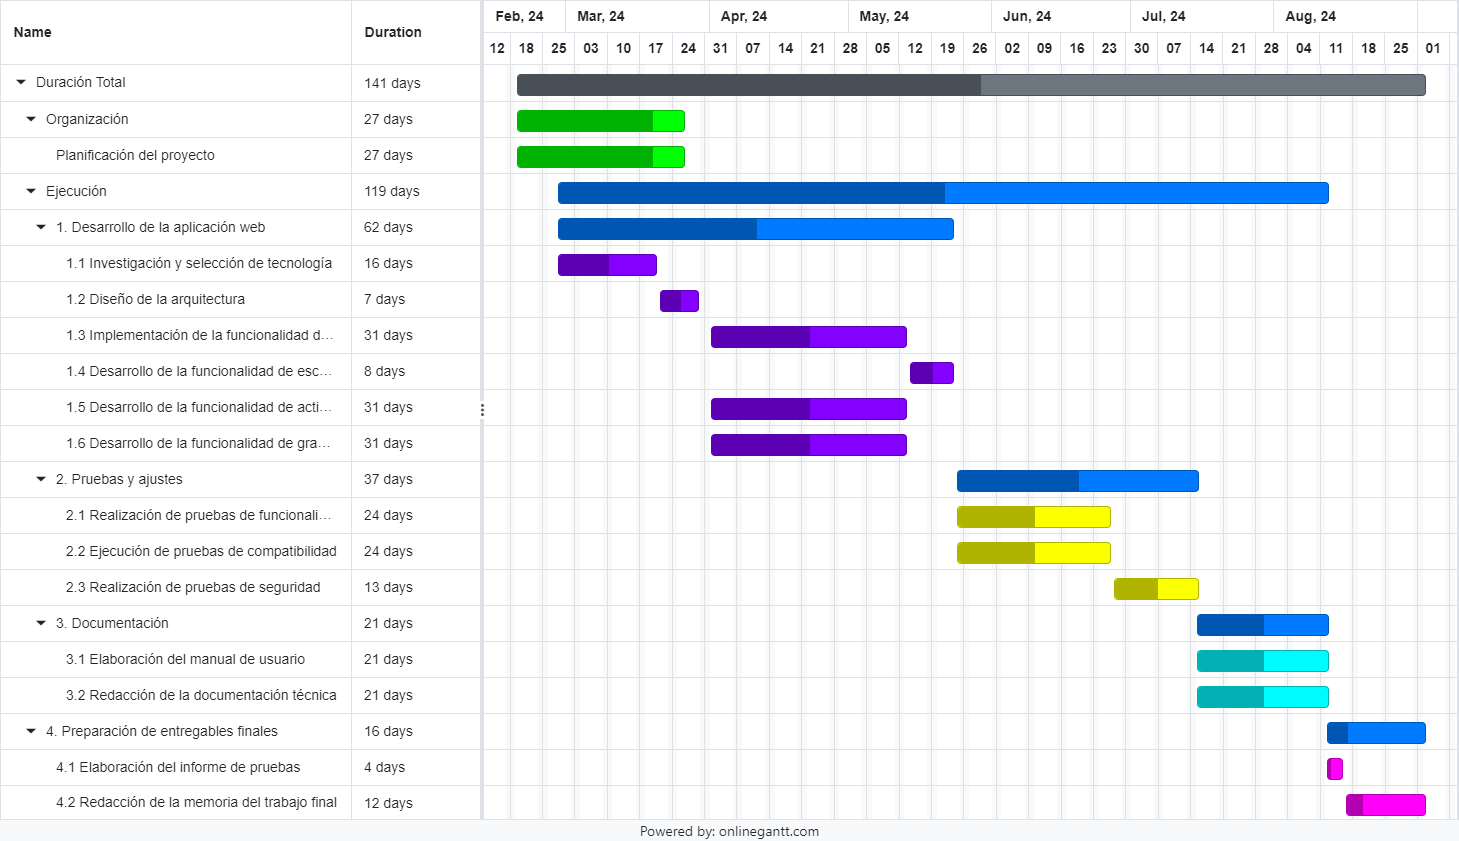
\includegraphics[width=.9\textwidth]{./Figuras/gantt.png}
    \caption{Diagrama Gantt del presente proyecto.}
    \label{fig:Gantt}
\end{sidewaysfigure}


\section{12. Presupuesto detallado del proyecto}
\label{sec:presupuesto}

El presupuesto del presente proyecto inicialmente fue calculado en dólares americanos. Sin embargo, bajo una tasa de cambio 1 USD = 856.74 ARS a la fecha del 26 de marzo de 2024, los valores equivalentes en la divisa argentina se muestran en la siguiente tabla.
\begin{table}[htpb]
\centering
\begin{tabularx}{\linewidth}{@{}|X|c|r|r|@{}}
\hline
\multicolumn{4}{|c|}{\cellcolor[HTML]{C0C0C0}COSTOS DIRECTOS} \\ \hline
\rowcolor[HTML]{C0C0C0} 
Descripción &
  \multicolumn{1}{c|}{\cellcolor[HTML]{C0C0C0}Cantidad} &
  \multicolumn{1}{c|}{\cellcolor[HTML]{C0C0C0}Valor unitario} &
  \multicolumn{1}{c|}{\cellcolor[HTML]{C0C0C0}Valor total} \\ \hline
 Horas de ingeniería. &
  \multicolumn{1}{c|}{520} &
  \multicolumn{1}{c|}{\$ 8138,97} &
  \multicolumn{1}{c|}{\$ 4232266,95} \\ \hline
 Componentes varios. &
  \multicolumn{1}{c|}{1} &
  \multicolumn{1}{c|}{\$ 1206.87} &
  \multicolumn{1}{c|}{\$ 1206.87} \\ \hline
\multicolumn{3}{|c|}{SUBTOTAL} &
  \multicolumn{1}{c|}{\$ 4352953,95} \\ \hline
\rowcolor[HTML]{C0C0C0} 
\multicolumn{4}{|c|}{\cellcolor[HTML]{C0C0C0}COSTOS INDIRECTOS} \\ \hline
\rowcolor[HTML]{C0C0C0} 
Descripción &
  \multicolumn{1}{c|}{\cellcolor[HTML]{C0C0C0}Cantidad} &
  \multicolumn{1}{c|}{\cellcolor[HTML]{C0C0C0}Valor unitario} &
  \multicolumn{1}{c|}{\cellcolor[HTML]{C0C0C0}Valor total} \\ \hline
Mes de alojamiento web. &
  \multicolumn{1}{c|}{6} &
  \multicolumn{1}{c|}{\$ 12851,13} &
  \multicolumn{1}{c|}{\$ 77106,78} \\ \hline
\multicolumn{3}{|c|}{SUBTOTAL} &
  \multicolumn{1}{c|}{\$ 77106,78} \\ \hline
\rowcolor[HTML]{C0C0C0}
\multicolumn{3}{|c|}{TOTAL} & \$ 4430060,73
   \\ \hline
\end{tabularx}%
\end{table}


\section{13. Gestión de riesgos}
\label{sec:riesgos}

\begin{consigna}{red}
a) Identificación de los riesgos (al menos cinco) y estimación de sus consecuencias:
 
Riesgo 1: detallar el riesgo (riesgo es algo que si ocurre altera los planes previstos de forma negativa)
\begin{itemize}
	\item Severidad (S): mientras más severo, más alto es el número (usar números del 1 al 10).\\
	Justificar el motivo por el cual se asigna determinado número de severidad (S).
	\item Probabilidad de ocurrencia (O): mientras más probable, más alto es el número (usar del 1 al 10).\\
	Justificar el motivo por el cual se asigna determinado número de (O). 
\end{itemize}   

Riesgo 2:
\begin{itemize}
	\item Severidad (S): X.\\
	Justificación...
	\item Ocurrencia (O): Y.\\
	Justificación...
\end{itemize}

Riesgo 3:
\begin{itemize}
	\item Severidad (S):  X.\\
	Justificación...
	\item Ocurrencia (O): Y.\\
	Justificación...
\end{itemize}


b) Tabla de gestión de riesgos:      (El RPN se calcula como RPN=SxO)

\begin{table}[htpb]
\centering
\begin{tabularx}{\linewidth}{@{}|X|c|c|c|c|c|c|@{}}
\hline
\rowcolor[HTML]{C0C0C0} 
Riesgo & S & O & RPN & S* & O* & RPN* \\ \hline
       &   &   &     &    &    &      \\ \hline
       &   &   &     &    &    &      \\ \hline
       &   &   &     &    &    &      \\ \hline
       &   &   &     &    &    &      \\ \hline
       &   &   &     &    &    &      \\ \hline
\end{tabularx}%
\end{table}

Criterio adoptado: 

Se tomarán medidas de mitigación en los riesgos cuyos números de RPN sean mayores a...

Nota: los valores marcados con (*) en la tabla corresponden luego de haber aplicado la mitigación.

c) Plan de mitigación de los riesgos que originalmente excedían el RPN máximo establecido:
 
Riesgo 1: plan de mitigación (si por el RPN fuera necesario elaborar un plan de mitigación).
  Nueva asignación de S y O, con su respectiva justificación:
  \begin{itemize}
	\item Severidad (S*): mientras más severo, más alto es el número (usar números del 1 al 10).
          Justificar el motivo por el cual se asigna determinado número de severidad (S).
	\item Probabilidad de ocurrencia (O*): mientras más probable, más alto es el número (usar del 1 al 10).
          Justificar el motivo por el cual se asigna determinado número de (O).
	\end{itemize}

Riesgo 2: plan de mitigación (si por el RPN fuera necesario elaborar un plan de mitigación).
 
Riesgo 3: plan de mitigación (si por el RPN fuera necesario elaborar un plan de mitigación).

\end{consigna}


\section{14. Gestión de la calidad}
\label{sec:calidad}

\begin{consigna}{red}
Elija al menos diez requerimientos que a su criterio sean los más importantes/críticos/que aportan más valor y para cada uno de ellos indique las acciones de verificación y validación que permitan asegurar su cumplimiento.

\begin{itemize} 
\item Req \#1: copiar acá el requerimiento con su correspondiente número.

\begin{itemize}
	\item Verificación para confirmar si se cumplió con lo requerido antes de mostrar el sistema al cliente. Detallar.
	\item Validación con el cliente para confirmar que está de acuerdo en que se cumplió con lo requerido. Detallar. 
\end{itemize}

\end{itemize}

Tener en cuenta que en este contexto se pueden mencionar simulaciones, cálculos, revisión de hojas de datos, consulta con expertos, mediciones, etc.  

Las acciones de verificación suelen considerar al entregable como ``caja blanca'', es decir se conoce en profundidad su funcionamiento interno.  

En cambio, las acciones de validación suelen considerar al entregable como ``caja negra'', es decir, que no se conocen los detalles de su funcionamiento interno.

\end{consigna}

\section{15. Procesos de cierre}    
\label{sec:cierre}

\begin{consigna}{red}
Establecer las pautas de trabajo para realizar una reunión final de evaluación del proyecto, tal que contemple las siguientes actividades:

\begin{itemize}
	\item Pautas de trabajo que se seguirán para analizar si se respetó el Plan de Proyecto original:\\
	 - Indicar quién se ocupará de hacer esto y cuál será el procedimiento a aplicar. 
	\item Identificación de las técnicas y procedimientos útiles e inútiles que se emplearon, los problemas que surgieron y cómo se solucionaron:\\
	 - Indicar quién se ocupará de hacer esto y cuál será el procedimiento para dejar registro.
	\item Indicar quién organizará el acto de agradecimiento a todos los interesados, y en especial al equipo de trabajo y colaboradores:\\
	  - Indicar esto y quién financiará los gastos correspondientes.
\end{itemize}

\end{consigna}
\end{document}